% to be compiled with: pdflatex --jobname=profile-f1 profile.tex
\documentclass[12pt]{book}
\usepackage[utf8]{inputenc}
\usepackage[T1]{fontenc}
\usepackage[frenchstyle,fulloldstylenums,partialup]{kpfonts}
\usepackage{tikz}
\usetikzlibrary{snakes}
%\pgfrealjobname{profile}
\begin{document}
\beginpgfgraphicnamed{profile-f1}
\footnotesize
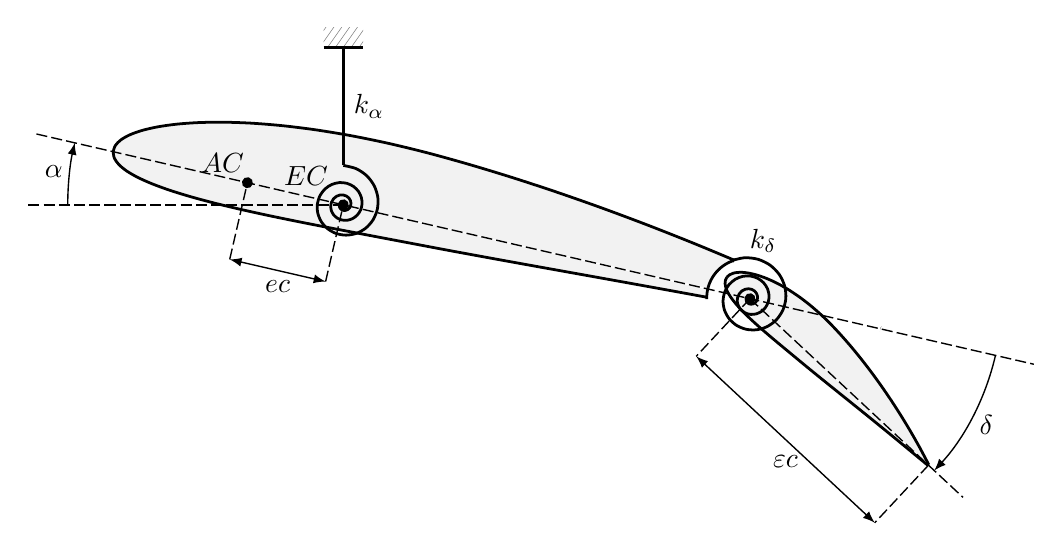
\begin{tikzpicture}[>=latex,scale=1]
\tikzstyle{spring}=[snake=zigzag,thick,line before snake=0.3cm,line after  snake=0.3cm,segment length=6,segment amplitude=5,join=round]%
\begin{scope}[rotate around={-13:(10,0)}]
% intrado
\draw[smooth,line width=1pt,fill=black!5] plot coordinates {(0,0)(0.0334,-0.0767)(0.1087,-0.1437)(0.2253,-0.2011)(0.3824,-0.2489)(0.5790,-0.2870)(0.8139,-0.3158)(1.0860,-0.3355)(1.3940,-0.3466)(1.7365,-0.3497)(2.1123,-0.3457)(2.5199,-0.3356) (2.9580,-0.3209)(3.4252,-0.3029)(3.9198,-0.2835)(4.4427,-0.2625)(4.9936,-0.2377)(5.5666,-0.2102)(6.1594,-0.1810)(6.7696,-0.1513)(7.3950,-0.1217)(8.0332,-0.0930)(8.6815,-0.0653)(9.3376,-0.0386)(9.9988,-0.0125)};
% extrado
\draw[smooth,line width=1pt,fill=black!5] plot coordinates {(0,0)(0.0095,0.0831)(0.0624,0.1691)(0.1590,0.2574)(0.2990,0.3467)(0.4824,0.4357)(0.7085,0.5225)(0.9765,0.6050)(1.2855,0.6812)(1.6341,0.7488)(2.0206,0.8055)(2.4433,0.8492)(2.8998,0.8778)(3.3879,0.8897)(3.9049,0.8833)(4.4459,0.8592)(5.0064,0.8210)(5.5876,0.7687)(6.1870,0.7023)(6.8016,0.6219)(7.4286,0.5277)(8.0650,0.4197)(8.7080,0.2980)(9.3544,0.1623)(10.0012,0.0125)};
% limits
\draw[line width=0.5pt,dashed,dash pattern=on 4pt off 1.5pt](3,-1)--(3,0);
\draw[line width=0.5pt,dashed,dash pattern=on 4pt off 1.5pt](1.75,-1)--(1.75,0);
\draw[line width=0.5pt,dashed,dash pattern=on 4pt off 1.5pt,rotate around={13:(3,0)}](-1,0)--(3,0);
% arrows
\draw[line width=0.5pt,<->](1.75,-1)--node[below]{$ec$}(3,-1);
\draw[line width=0.5pt,<-](3,0) +(180:3.5cm) arc (180:193:3.5cm);
\draw(3,0) +(186.5:3.7cm) node{$\alpha$};
% points
\fill(3,0)circle (2pt);
\draw(3,0)+(155:0.6cm) node{$EC$};
\fill(1.75,0) circle (2pt);
\draw(1.75,0)+(155:0.4cm) node{$AC$};
\begin{scope}[xshift=3cm,rotate=103]
\draw [domain=0:25.1327,variable=\t,smooth,samples=75,line width=1pt]plot ({\t r}:{0.0008*\t*\t});
\end{scope}
\draw[rotate around={13:(3,0)},line width=1pt](3,0.5)--node[right]{$k_\alpha$} (3,2);%
\begin{scope}[rotate around={13:(3,0)}]
\clip (2.75,2) rectangle (3.25,2.25);
\foreach \x in {2.5,2.6,...,5} {
\draw[gray,line width=0.2pt](\x,2)--+(55:2);}
\end{scope}%
\draw[line width=1pt,rotate around={13:(3,0)}] (2.75,2) -- (3.25,2);
\draw[fill=white,white] (8.25,0) --+(0:.5) arc (0:360:.5);
\draw[line width=1pt] (8.25,0) --+(120:.5) arc (120:195:.5);
\fill[fill=white] (8,-.25) rectangle (10,.5);
% winglet
\begin{scope}[rotate around={-30:(8.3,0)},xshift=7.9cm,scale=0.35,y=1.5cm]
% intrado
\draw[smooth,line width=1pt,fill=black!5] plot coordinates {(0,0)(0.0334,-0.0767)(0.1087,-0.1437)(0.2253,-0.2011)(0.3824,-0.2489)(0.5790,-0.2870)(0.8139,-0.3158)(1.0860,-0.3355)(1.3940,-0.3466)(1.7365,-0.3497)(2.1123,-0.3457)(2.5199,-0.3356) (2.9580,-0.3209)(3.4252,-0.3029)(3.9198,-0.2835)(4.4427,-0.2625)(4.9936,-0.2377)(5.5666,-0.2102)(6.1594,-0.1810)(6.7696,-0.1513)(7.3950,-0.1217)(8.0332,-0.0930)(8.6815,-0.0653)(9.3376,-0.0386)(9.9988,-0.0125)};
% extrado
\draw[smooth,line width=1pt,fill=black!5] plot coordinates {(0.0000,0.0000)(0.0095,0.0831)(0.0624,0.1691)(0.1590,0.2574)(0.2990,0.3467)(0.4824,0.4357)(0.7085,0.5225)(0.9765,0.6050)(1.2855,0.6812)(1.6341,0.7488)(2.0206,0.8055)(2.4433,0.8492)(2.8998,0.8778)(3.3879,0.8897)(3.9049,0.8833)(4.4459,0.8592)(5.0064,0.8210)(5.5876,0.7687)(6.1870,0.7023)(6.8016,0.6219)(7.4286,0.5277)(8.0650,0.4197)(8.7080,0.2980)(9.3544,0.1623)(10.0012,0.0125)};
\end{scope}
\draw[line width=0.5pt,dashed,dash pattern=on 4pt off 1.5pt,rotate around={-30:(8.3,0)}](8.3,0)--(12,0);
\draw[line width=0.5pt,dashed,dash pattern=on 4pt off 1.5pt,rotate around={-30:(8.3,0)}](8.3,0)--(8.3,-1);
\draw[line width=0.5pt,dashed,dash pattern=on 4pt off 1.5pt,rotate around={-30:(8.3,0)}](11.4,0)--(11.4,-1);
\draw[line width=0.5pt,rotate around={-30:(8.3,0)},<->](8.3,-1)--node[below]{$\vphantom{6}\varepsilon c$}(11.4,-1);
\fill(8.3,0)circle (2pt);
\begin{scope}[xshift=8.3cm,rotate=130]
\draw [domain=0:25.1327,variable=\t,smooth,samples=75,line width=1pt]plot ({\t r}:{0.00085*\t*\t});
\end{scope}
\draw(8.3,0)+(90:0.75cm) node{$k_\delta$};
\draw[line width=0.5pt,<-](8.3,0) +(330:3.2cm) arc (330:360:3.2cm);
\draw(8.3,0) +(345:3.4cm) node{$\delta$};
\draw[line width=0.5pt,dashed,dash pattern=on 4pt off 1.5pt](-1,0)--(12,0);
\end{scope}%
\end{tikzpicture}
\endpgfgraphicnamed%
\end{document}